\section{Fonctions à connaître dès le début}
\label{sec:fonctiondebut}

Je ne prendrai pas le temps de décrire chaque touche de la calculatrice, tout le monde sait déjà comment fonctionne une calculatrice scientifique. Donc, voici les quelques fonctions que je ne connaissais pas au début mais que j'aime bien.

\subsection{Décimal à fraction}
Une touche toute simple que j'ai connu trop tard: La touche \raisebox{-1mm}{
\includegraphics[height=5mm]{B_FlechesOpposees}} %avec deux flèches opposées
au-dessus de la touche \texttt{enter} (en bas à droite). Elle sert à convertir le format d'une réponse entre nombre à virgule et fraction.

\subsection{Les fonctions de probabilité}
Le bouton \raisebox{-1mm}{
\includegraphics[height=5mm]{B_Prb}} permet de faire des combinaisons, des permutations et des factoriels. Rien de compliqué, il faut simplement l'essayer (pour les combinaisons ${n \choose x}$, on doit mettre \texttt{n}, puis pèser sur \raisebox{-1mm}{
\includegraphics[height=5mm]{B_Prb}}, puis \texttt{2}, et finalement \texttt{x}. Si tu ne sais pas encore ce qu'est une combinaison ou un factoriel, tu vas le savoir bien assez vite.

\subsection{Garder une valeur en mémoire}
Je pense que la seule fois que j'ai utilisé cette fonction, c'était avec la fonction \texttt{Table} décrite plus loin afin de changer plus facilement le paramètre d'une loi (fonction de survie de la Gompertz dans un examen papier trop long en vie I). La fonction peut aussi servir lors des examens professionnels quand on est habitué d'avoir plein de numéros semblables avec les mêmes variables, pour stocker un taux d'intérêt par exemple.

Pour garder une valeur en mémoire, on entre cette valeur (ou elle sera déjà entrée parce que c'est le résultat d'un calcul), puis on appuie sur \raisebox{-1mm}{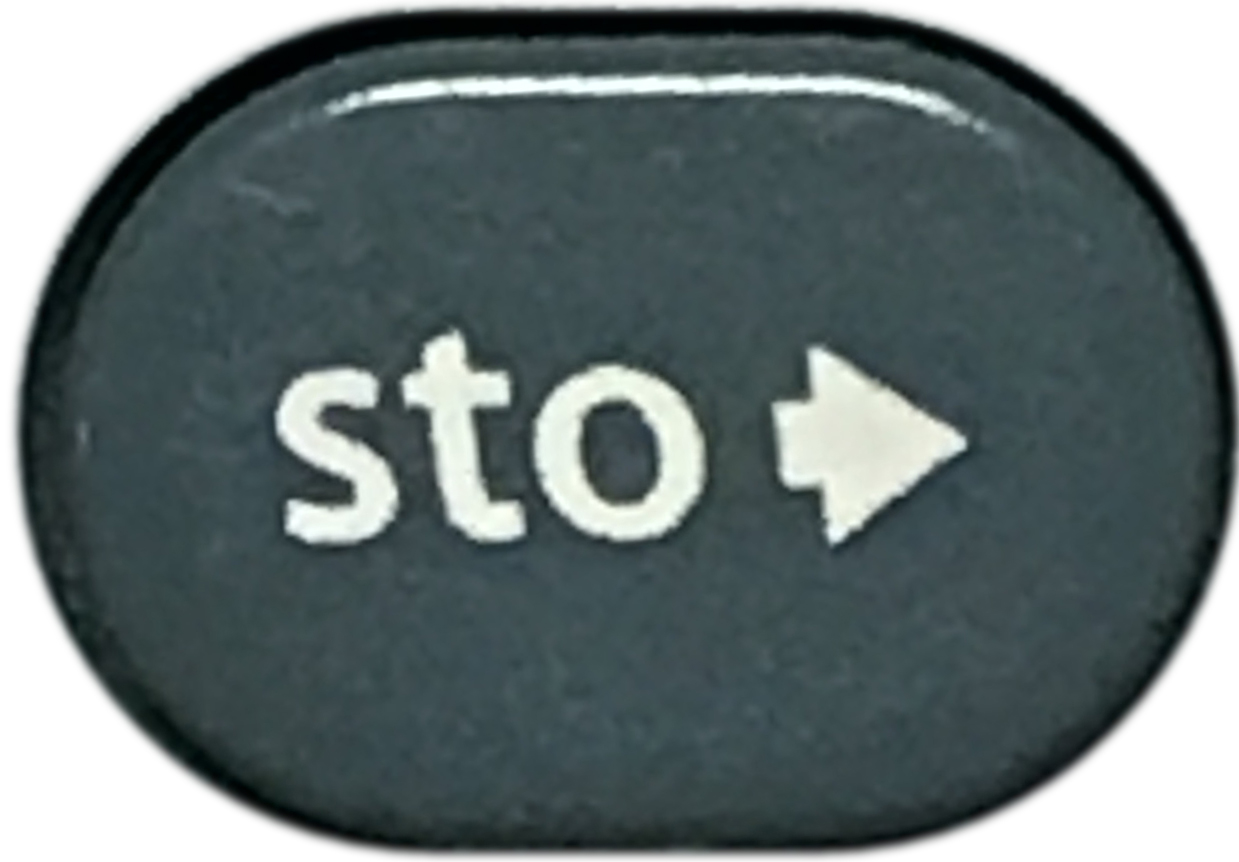
\includegraphics[height=5mm]{B_Sto}} pour dire qu'on veut la sauvegarder. Finalement, on appuie sur \raisebox{-1mm}{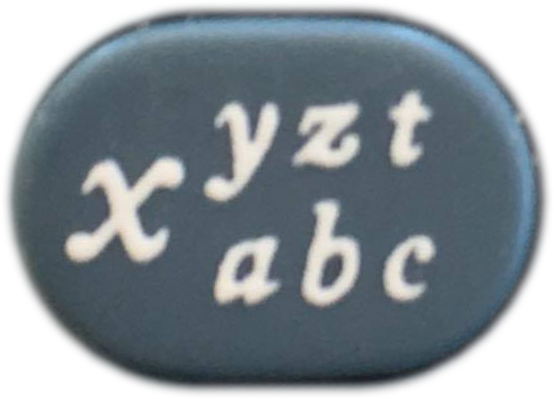
\includegraphics[height=5mm]{B_Xyztabc}} pour choisir quelle lettre représentera la valeur. Pour voir le contenu de chaque variable ou la réutiliser, on pèse sur \raisebox{-1mm}{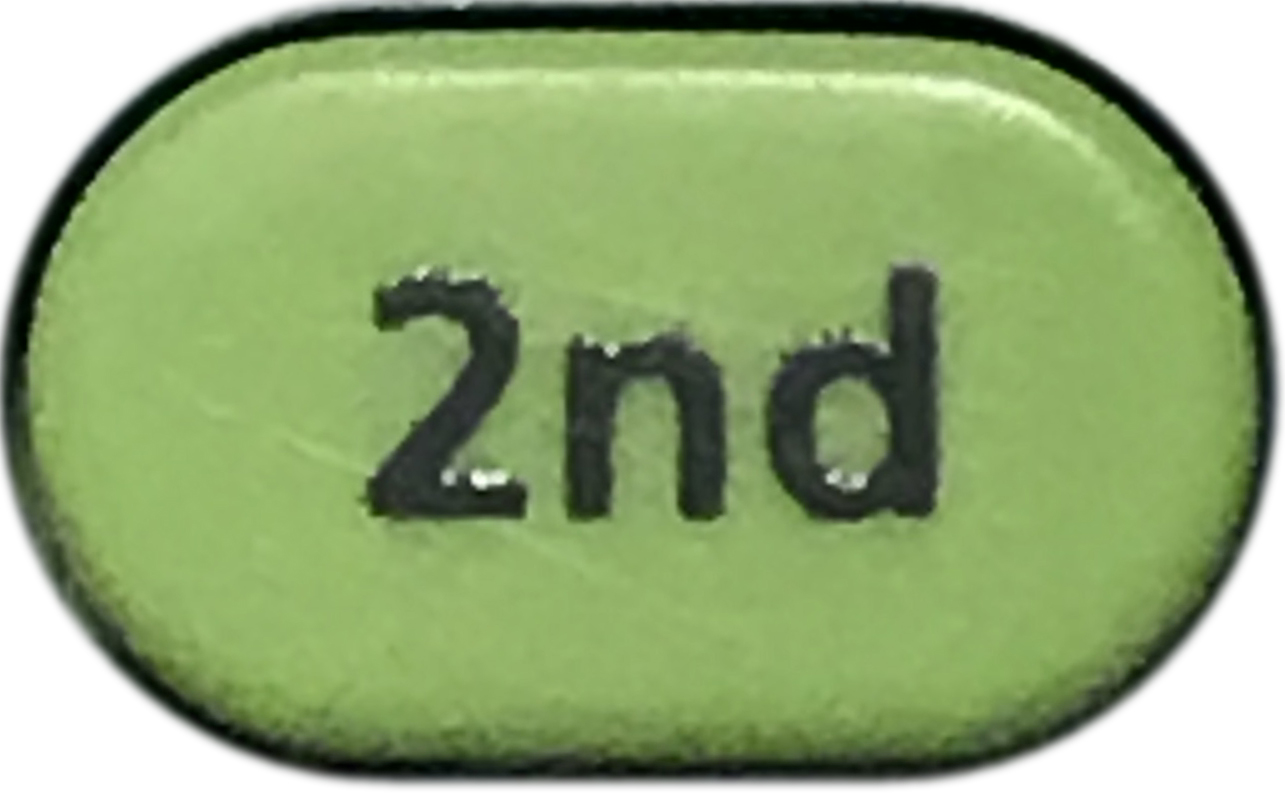
\includegraphics[height=5mm]{B_2nd}} et \raisebox{-1mm}{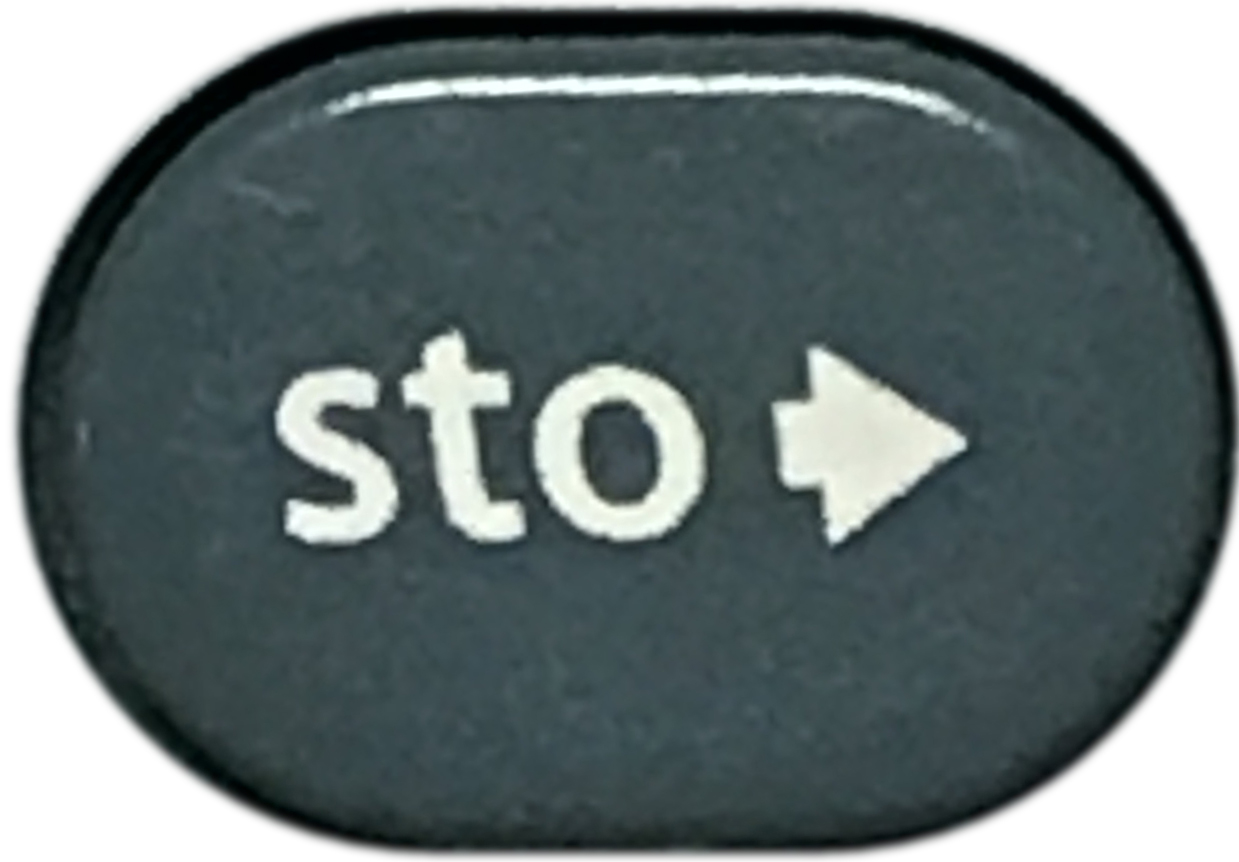
\includegraphics[height=5mm]{B_Sto}}. Pour la réutiliser plus rapidement, on pèse sur \raisebox{-1mm}{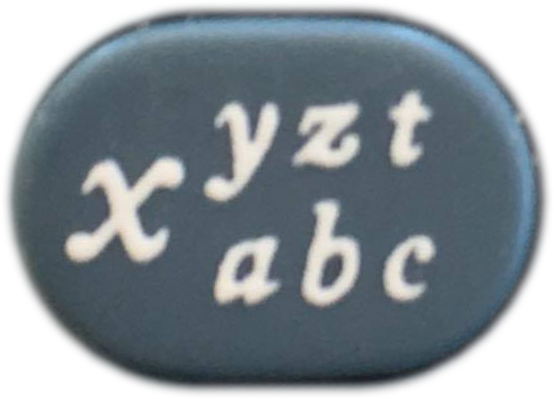
\includegraphics[height=5mm]{B_Xyztabc}} jusqu'à ce que ça sorte la bonne variable.

Pour revenir à mon exemple, c'est que la formule à entrer était trop longue pour être mise dans la fonction \texttt{Table} et j'avais à calculer pour plusieurs valeurs d'un paramètre. J'ai donc pu faire un \texttt{Recall} de \texttt{x} dans ma formule dans \texttt{Table} et changer la valeur de \texttt{x} avec cette méthode.

\subsection{La fonction \texttt{Table}}
Cette fonction sert à essayer plusieurs valeurs de \texttt{x} dans une fonction mathématique. Par exemple, je m'en suis servis en Compléments de mathématiques pour trouver les racines d'une fonction ou dans les examens professionnels pour essayer les différents choix de réponse. 

Pour s'en servir, on pèse sur \raisebox{-1mm}{
\includegraphics[height=5mm]{B_Table}} et on entre la fonction de \texttt{x}, le bouton \raisebox{-1mm}{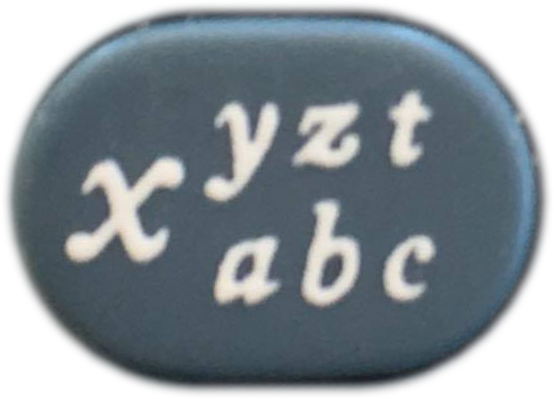
\includegraphics[height=5mm]{B_Xyztabc}} sert à mettre les \texttt{x}. Ensuite, après avoir pesé sur \texttt{enter}, il y aura différentes options pour décider des valeurs de x à entrer, rien de trop compliqué.

\subsection{La fonction \texttt{Data}}
La fonction \texttt{Data} est celle que je me sers le plus souvent, mais il faut prendre le temps d'apprendre à bien l'utiliser. C'est dur d'expliquer clairement dans quels cas elle peut servir, donc je vais me contenter de l'expliquer.

On appuie sur \raisebox{-1mm}{
\includegraphics[height=5mm]{B_Data}} pour voir les trois colonnes de la fonction \texttt{Data}. Dans chacune des colonnes (on utilise \raisebox{-2.5mm}{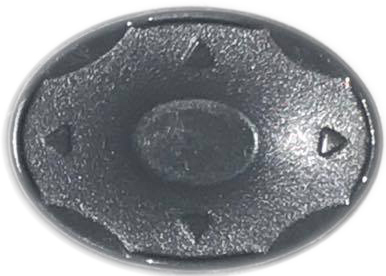
\includegraphics[height=7mm]{B_4Fleches}} pour sélectionner les différentes cellules), on peut entrer des nombres ou des formules qui dépendent des autres colonnes.

On appuie encore sur \raisebox{-1mm}{
\includegraphics[height=5mm]{B_Data}} pour accéder au menu de \texttt{Data}. Ici, on peut effacer le contenu d'une colonne ou de toutes en descendant dans les options. On peut aussi utiliser le nombre à gauche pour sélectionner une option (on appuie sur \texttt{1} pour effacer le contenu de la première colonne). Sinon, en haut de l'écran, à droite de \texttt{CLEAR}, il y a \texttt{FORMULA}. En y allant et en sélectionnant la première option (\texttt{Add/Edit Frmla}), on peut entrer une formule dans la colonne où on était. 

On peut maintenant entrer la formule qui peut être fonction des deux autres colonnes (mais seulement sur une même ligne. Par exemple, on ne peut pas entrer une formule en fonction de la cellule au-dessus). Pour mettre la valeur d'une autre colonne dans la formule, on appuie une troisième fois sur \raisebox{-1mm}{
\includegraphics[height=5mm]{B_Data}} et on choisit la bonne colonne.

\section{Fonctions statistiques}

On entre dans une section qui ne sera pas vraiment utile pour les étudiants en première session. Je pense que les fonctions statistiques de la calculatrice vont surtout servir pour les cours de statistiques (2e session), IARD I, Modèles linéaires (3e session) et IARD II (4e session), en plus des examens MFE et C.

\subsection{Entrer des données}
\label{subsec:EntrerDonnees}

Pour entrer les données, on utilise la fonction \texttt{data}, déjà présentée à la \autoref{sec:fonctiondebut}. De mémoire, il y a trois façons de recevoir des données dans une questions:

\begin{enumerate}

\item Chaque donnée est différente, ex: (10, 12, 15, 20)
\label{itm:donneedifferente}

\item Les données sont répétées, ex: (2, 2, 2, 4, 4, 7, 7, 7, 7, 7, 7, 7)
\label{itm:donneerepetee}

\item On a une variable explicative \texttt{x} et une variable réponse \texttt{y}, donc chaque observation a deux données associées
\label{itm:donneeassociee}

\end{enumerate}

La \autoref{itm:donneedifferente} est intuitive. On entre les données dans une colonne, tout simplement.

Pour la \autoref{itm:donneerepetee}, on entre les valeurs dans une colonne et le nombre de répétition de chaque valeur dans une autre colonne.

La \autoref{itm:donneeassociee} est liée au cours de modèles linéaires. Les fonctions statistiques à deux variables seront présentées dans la sous-section \nameref{subsec:statdeuxvariables}.

\subsection{Utiliser \texttt{Stat} avec une variable}

Une fois que les données sont entrées dans \texttt{data}, il ne reste qu'à appuyer sur \raisebox{-1mm}{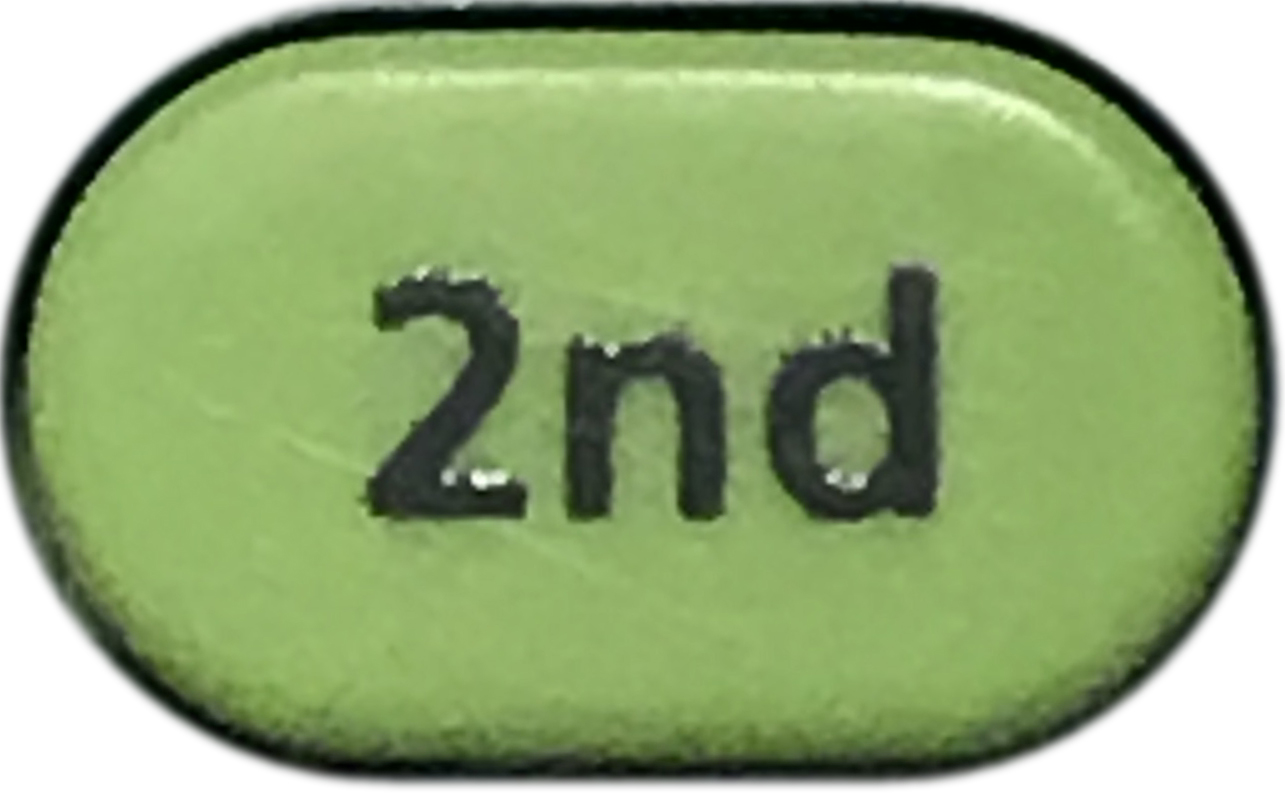
\includegraphics[height=5mm]{B_2nd}} et \raisebox{-1mm}{
\includegraphics[height=5mm]{B_Data}}, puis à sélectionner \texttt{1: 1-Var Stats}. On choisit ensuite comment les données étaient entrées, donc dans quelle colonne étaient les données et, pour la \autoref{itm:donneerepetee} (où les données sont répétées), on choisit dans \texttt{FRQ:} la colonne qui donne le nombre de fois que chaque donnée est répétée.

C'est tout! On a maintenant accès à toutes ces statistiques:

\begin{desclist}{\sf}{ \rm\hfill}[minX]

\item [n] nombre d'observations
\item [x] moyenne empirique
\item [Sx] variance empirique non biaisée (divisée par ${n - 1}$)
\item [$\sigma_{x}$] variance empirique biaisée (divisée par ${n}$)
\item [$\sum x$] somme des observations
\item [$\sum x^{2}$] somme des observations au carré
\item [minX] minimum des observations
\item [\ldots]

\end{desclist}



\subsection[Utiliser \texttt{Stat} avec deux variables]{Utiliser \texttt{Stat} avec deux variables (modèles linéaires)}
\label{subsec:statdeuxvariables}

Pour utiliser les fonctions de statistiques à deux variables, liées à un modèle de régression linéaire simple que l'on voit dans le cours de modèles linéaires à la 3e session, il faut d'abord entrer les différentes observations comme à la \ref{subsec:EntrerDonnees}. J'utiliserai la notation $\hat{Y_i} = \beta_0 + \beta_1 \cdot X_i$, donc $X$ est la variable explicative et $Y$ la variable réponse.

Donc, une fois les $X$ entrés dans une colonne et les $Y$ dans une autre (dans \texttt{data}), on pèse sur \raisebox{-1mm}{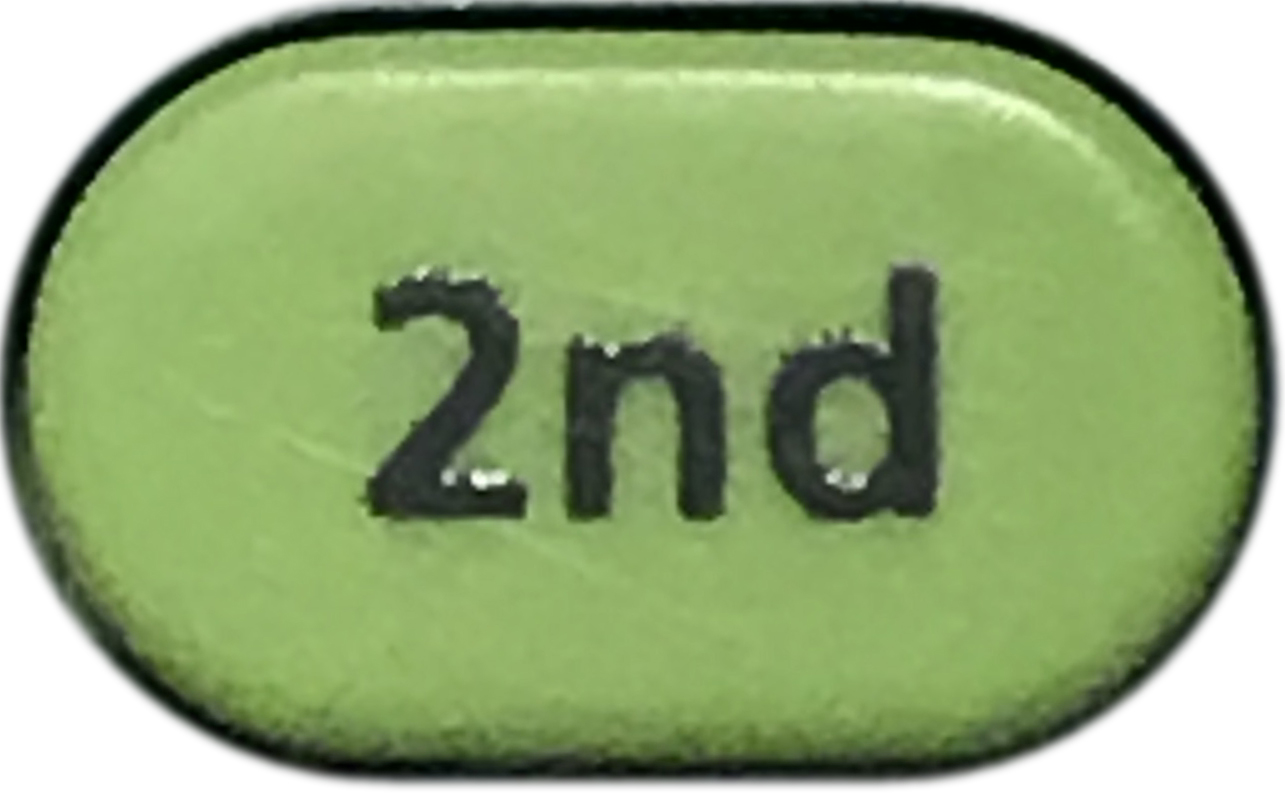
\includegraphics[height=5mm]{B_2nd}} et \raisebox{-1mm}{
\includegraphics[height=5mm]{B_Data}}. Ensuite, on choisit \texttt{2: 2-Var Stats} et on indique à la calculatrice quelle colonne est associée à quelle variable.

Terminé! Je veux juste faire remarquer les statistiques qui peuvent être très pratiques:

\begin{desclist}{\sf}{ \rm\hfill}[minX]

\item [a] Valeur de $\beta_1$
\item [b] Valeur de $\beta_0$
\item [r] Mis au carré, ça nous donne $R^2$
\item [x'] Donne la valeur de $X_i$ qui serait associée à la valeur de $Y_i$ qu'on entre après avoir sélectionné cette fonction
\item [y'] Même principe, on choisit cette fonction puis on entre une valeur de $X_i$, ça sors la valeur prédite de $Y_i$

\end{desclist}